\documentclass{article}

\title{Efficient low rank approximation with affine embeddings}
\author{Kadin Zhang}
\date{15-851, Spring 2025}

\usepackage[dvipsnames]{xcolor}
\usepackage{tikz}
\usetikzlibrary{calc}
\usepackage{enumitem}
\usepackage{alltt}
\usepackage{amsfonts}
\usepackage{amsmath}
\usepackage{amssymb}
\usepackage{amsthm}
\usepackage{booktabs}
\usepackage{bm}
\usepackage{bbm}
\usepackage{caption}
\usepackage{graphicx}
\usepackage{mathrsfs}
\usepackage{mathdots}
\usepackage{mathtools}
\usepackage{microtype}
\usepackage{multirow}
\usepackage{soul}
\usepackage{empheq}
\usepackage{mdframed}

% mdframed environments remain unchanged:
\newmdenv[
  innerbottommargin = 4mm,
  middlelinewidth = 0.3mm,
  linecolor = darkgray,
  backgroundcolor=TealBlue!10,
  nobreak=true
]{boxexample}
\newenvironment{ex}{\boxexample\begin{eg}}{\end{eg}\endboxexample}

\newmdenv[
  innerbottommargin = 4mm,
  middlelinewidth = 0.3mm,
  linecolor = darkgray,
  backgroundcolor=Salmon!10,
  nobreak=true
]{boxtheo}

\newmdenv[
  innerbottommargin = 4mm,
  middlelinewidth = 0.3mm,
  linecolor = darkgray,
  backgroundcolor=Goldenrod!20,
  nobreak=true
]{boxdefinition}
\newenvironment{thm}{\boxtheo\begin{theo}}{\end{theo}\endboxtheo}
\newenvironment{boxdef}{\boxdefinition\begin{defi}}{\end{defi}\endboxtheo}

\newenvironment{enum}{\newblock\begin{enumerate}[label=(\alph*)]}{\end{enumerate}}
\newenvironment{statement}[1]{\smallskip\noindent\color{BrickRed} {\bf #1.}}{}
\newenvironment{prob}{\color{BrickRed}\begin{probinner}}{\end{probinner}}
\newenvironment{comments}{\color{BrickRed}\begin{commentinner}}{\end{commentinner}}
\usepackage{imakeidx}
\newcommand{\argmin}{\operatornamewithlimits{arg\,min}}
\newcommand{\argmax}{\operatornamewithlimits{arg\,max}}

\makeindex[intoc, title=Index]
\usepackage[pdftex,
  hidelinks,
  pdfauthor={Kadin Zhang},
  pdfsubject={},
  pdftitle={},
  pdfkeywords={}]{hyperref}
\renewcommand\printindex{}

% Set standard 1-inch margins using the geometry package.
\usepackage[margin=1in]{geometry}

% Theorem styles and macros:
\newtheoremstyle{definition}{}{}{}{}{\bfseries}{:}{.5em}{\thmname{#1}\thmnumber{ #2}\thmnote{ (\textcolor{darkgray}{#3})}}
\theoremstyle{definition}

\newtheorem*{aim}{Aim}
\newtheorem*{axiom}{Axiom}
\newtheorem*{claim}{Claim}
\newtheorem*{cor}{Corollary}
\newtheorem*{conjecture}{Conjecture}
\newtheorem*{commentinner}{Comments}
\newtheorem*{defi}{Definition}
\newtheorem*{eg}{Example}
\newtheorem*{exc}{Exercise}
\newtheorem*{fact}{Fact}
\newtheorem*{law}{Law}
\newtheorem*{lemma}{Lemma}
\newtheorem*{notation}{Notation}
\newtheorem*{prop}{Proposition}
\newtheorem*{question}{Question}
\newtheorem*{rrule}{Rule}
\newtheorem*{theo}{Theorem}
\newtheorem*{assumption}{Assumption}

\newtheorem*{remark}{Remark}
\newtheorem*{warning}{Warning}
\newtheorem*{exercise}{Exercise}

\newtheorem{nthm}{Theorem}[section]
\newtheorem{nlemma}[nthm]{Lemma}
\newtheorem{nprop}[nthm]{Proposition}
\newtheorem{ncor}[nthm]{Corollary}
\newtheorem{probinner}[nthm]{Problem}

\renewcommand{\labelitemi}{--}
\renewcommand{\labelitemii}{$\circ$}
\renewcommand{\labelenumi}{(\roman{*})}

\newcommand\qedsym{\hfill\ensuremath{\square}}
\def\st{\bgroup \ULdepth=-.55ex \ULset}

% Mathematics symbols and operator definitions:
\newcommand{\leb}{\text{Leb}}

\newcommand{\C}{\mathbb{C}}
\newcommand{\CP}{\mathbb{CP}}
\newcommand{\GG}{\mathbb{G}}
\newcommand{\N}{\mathbb{N}}
\newcommand{\F}{\mathbb{F}}
\newcommand{\Q}{\mathbb{Q}}
\newcommand{\R}{\mathbb{R}}
\newcommand{\RP}{\mathbb{RP}}
\newcommand{\T}{\mathbb{T}}
\newcommand{\Z}{\mathbb{Z}}
\renewcommand{\H}{\mathbb{H}}

\DeclarePairedDelimiter\parens{\lparen}{\rparen}
\DeclarePairedDelimiter\abs{\lvert}{\rvert}
\DeclarePairedDelimiter\norm{\lVert}{\rVert}
\DeclarePairedDelimiter\floor{\lfloor}{\rfloor}
\DeclarePairedDelimiter\ceil{\lceil}{\rceil}
\DeclarePairedDelimiter\braces{\lbrace}{\rbrace}
\DeclarePairedDelimiter\bracks{\lbrack}{\rbrack}
\DeclarePairedDelimiter\angles{\langle}{\rangle}

\DeclarePairedDelimiter\bigp{\Big(}{\Big)}
\DeclarePairedDelimiter\bigc{\Bigg\{}{\Bigg\}}
\DeclarePairedDelimiter\biga{\Bigg|}{\Bigg|}

\DeclareMathOperator{\poly}{poly}
\DeclareMathOperator{\polylog}{polylog}
\DeclareMathOperator{\size}{size}
\DeclareMathOperator{\sgn}{sgn}
\DeclareMathOperator{\dist}{dist}
\DeclareMathOperator{\vol}{vol}
\DeclareMathOperator{\spn}{span}
\DeclareMathOperator{\supp}{supp}
\DeclareMathOperator{\tr}{tr}
\DeclareMathOperator{\Tr}{Tr}
\DeclareMathOperator{\codim}{codim}
\DeclareMathOperator{\diag}{diag}

\DeclareMathOperator{\lcm}{lcm}
\DeclareMathOperator{\OPT}{OPT}
\DeclareMathOperator{\DFT}{DFT}
\DeclareMathOperator{\rank}{rank}
\DeclareMathOperator{\nul}{nul}
\DeclareMathOperator{\ord}{ord}
\DeclareMathOperator{\diam}{diam}
\DeclareMathOperator{\erf}{erf}
\DeclareMathOperator{\err}{err}
\newcommand{\eps}{\varepsilon}

\DeclareMathOperator{\adj}{adj}
\DeclareMathOperator{\Aut}{Aut}
\DeclareMathOperator{\Char}{char}
\DeclareMathOperator{\Hom}{Hom}
\DeclareMathOperator{\id}{id}
\DeclareMathOperator{\image}{image}
\DeclareMathOperator{\im}{im}
\newcommand{\Frob}{\mathrm{Frob}}

\newcommand{\bolds}[1]{{\bfseries #1}}
\newcommand{\cat}[1]{\mathsf{#1}}
\newcommand{\mc}[1]{\mathcal{#1}}
\newcommand{\ph}{\,\cdot\,}
\newcommand{\term}[1]{\emph{#1}\index{#1}}
\newcommand{\phantomeq}{\hphantom{{}={}}}

\DeclareMathOperator{\PoA}{PoA}
\DeclareMathOperator{\PoS}{PoS}
\DeclareMathOperator{\Ber}{Ber}
\DeclareMathOperator{\io}{i.o.}
\DeclareMathOperator{\ev}{ev}
\DeclareMathOperator{\U}{U}
\DeclareMathOperator{\betaD}{beta}
\DeclareMathOperator{\bias}{bias}
\DeclareMathOperator{\Bin}{Bin}
\DeclareMathOperator{\corr}{corr}
\DeclareMathOperator{\cov}{cov}
\DeclareMathOperator{\var}{var}
\DeclareMathOperator{\gammaD}{gamma}
\DeclareMathOperator{\mse}{mse}
\DeclareMathOperator{\multinomial}{multinomial}
\DeclareMathOperator{\Poisson}{Poisson}
\newcommand{\E}{\mathbf{E}}
\newcommand{\wto}{\rightharpoonup}
\newcommand{\dto}{\xrightarrow{\text{d}}}
\newcommand{\pto}{\xrightarrow{\text{p}}}
\newcommand{\ato}{\xrightarrow{\text{a.s.}}}

\let\P\relax
\newcommand{\P}{\mathbf{P}}
\let\Pr\relax
\DeclareMathOperator*{\Pr}{\mathbf{Pr}}

\let\Im\relax
\let\Re\relax

\makeatother


\begin{document}
\maketitle
{
\small
\setlength{\parindent}{0em}
\setlength{\parskip}{1em}
}

Let $A$ be a large $n\times d$ matrix, like a customer-product matrix. Typically these are well approximated by lower rank matrices, which take much less parameters to store (we can store a $n\times k$ matrix and a $k\times d$ matrix), and have the added benefit of denoising.

We can solve for the best rank $k$ approximation to $A$ in closed form with SVD: 
\begin{thm}[Truncated SVD is optimal low rank approximation]
    Let $A_k = U \Sigma _k V^{\top}  $, where $\Sigma_k  $ zeros all singular values outside of the top $k$. Then 
    \[
        A_k  = \argmin_{\rank (B) = k} \norm*{B - A}_{F}  
    \]
\end{thm}
The problem is that SVD will cost $O(nd^2 )$, which is intractible when $n$ and $d$ are large. We will show that we can get a rank $k$ approximation $A'$ with 
\[
    \norm*{A' - A}_{F} \leq (1+\eps )\norm*{A_k -A}_{F} ,
\]
with constant probability of failure in $O(nnz(A) + (n+d)\poly(d/\eps ))$ time. We will make use of affine embeddings: 
\begin{defi}[Affine embedding]
    Let $A$ be a $n\times d$ and $B$ be $n \times m$. We wish to solve the regression problem
    \[
        \min _X \norm*{AX-B}_{F} ^2 . 
    \]
    An \emph{affine embedding} is a short matrix $S$ such that for all $X$, 
    \[
        \norm*{S(AX-B)}_{F} \leq (1+\eps )\norm*{AX-B}_{F}
    \]
    holds with constant probability. CountSketch matrices of dimension $O(d^2 /\eps ^2 ) \times n $ are one such family that satisfy the affine embedding property.
\end{defi}

\section{Motivation}
We would like to output a rank matrix $A'$ such that 
\[
    \norm*{A - A'}_{F} \leq (1+\eps ) \norm*{A- A_k }_{F} .
\]
As motivation, consider the regression problem $\min _X \norm*{A_k X-A}_{F} $ with optimum $X^* = I$, and an affine embedding $S$. The property of $S$ tells us for all $X$:
\[
    \norm*{SA_k X- SA}_{F} \leq (1+\eps ) \norm*{A_k X- A}_{F}.
\]
The optimal $X$ for the LHS is $X' = (SA_k )^- SA$, which is in the rowspan of $SA$. Since $S$ is an affine embedding, the sketched optimum is a good approximation:
\begin{align*}
    (1-\eps )\norm*{A_k X' - A}_F  &\leq \norm*{SA_k X' - SA}_{F} \\
    &\leq  \norm*{SA_k X^* - SA}_{F}\\
     &\leq (1+\eps ) \norm*{A_k X^*  - A}_{F} \\
     &= (1+\eps ) \norm*{A_k -A}_{F} . 
\end{align*}
In conclusion, $A_k (SA_k )^- SA$ is a good rank $k$ approximation to $A_k $ in the rowspan of $SA$. 

This outlines an initial strategy: 
\begin{enum}
    \item Choose a $k/\eps \times n$ sketching matrix $S$. We assume CountSketch henceforth, since this allows us to compute $SA$ in $O(nnz(A))$. 
    \item Find a rank $k$ approximation with SVD within the rowspan of $SA$ rather than $A$. We can think of $SA$ through rows: each row is a random linear combination of rows of $A$, which live in $\R^d $. But the rows of $SA$ are now in a $k/\eps $-dimensional subspace, so we have ``projected'' the rows of $A$ onto $SA$: 
     \begin{center}
        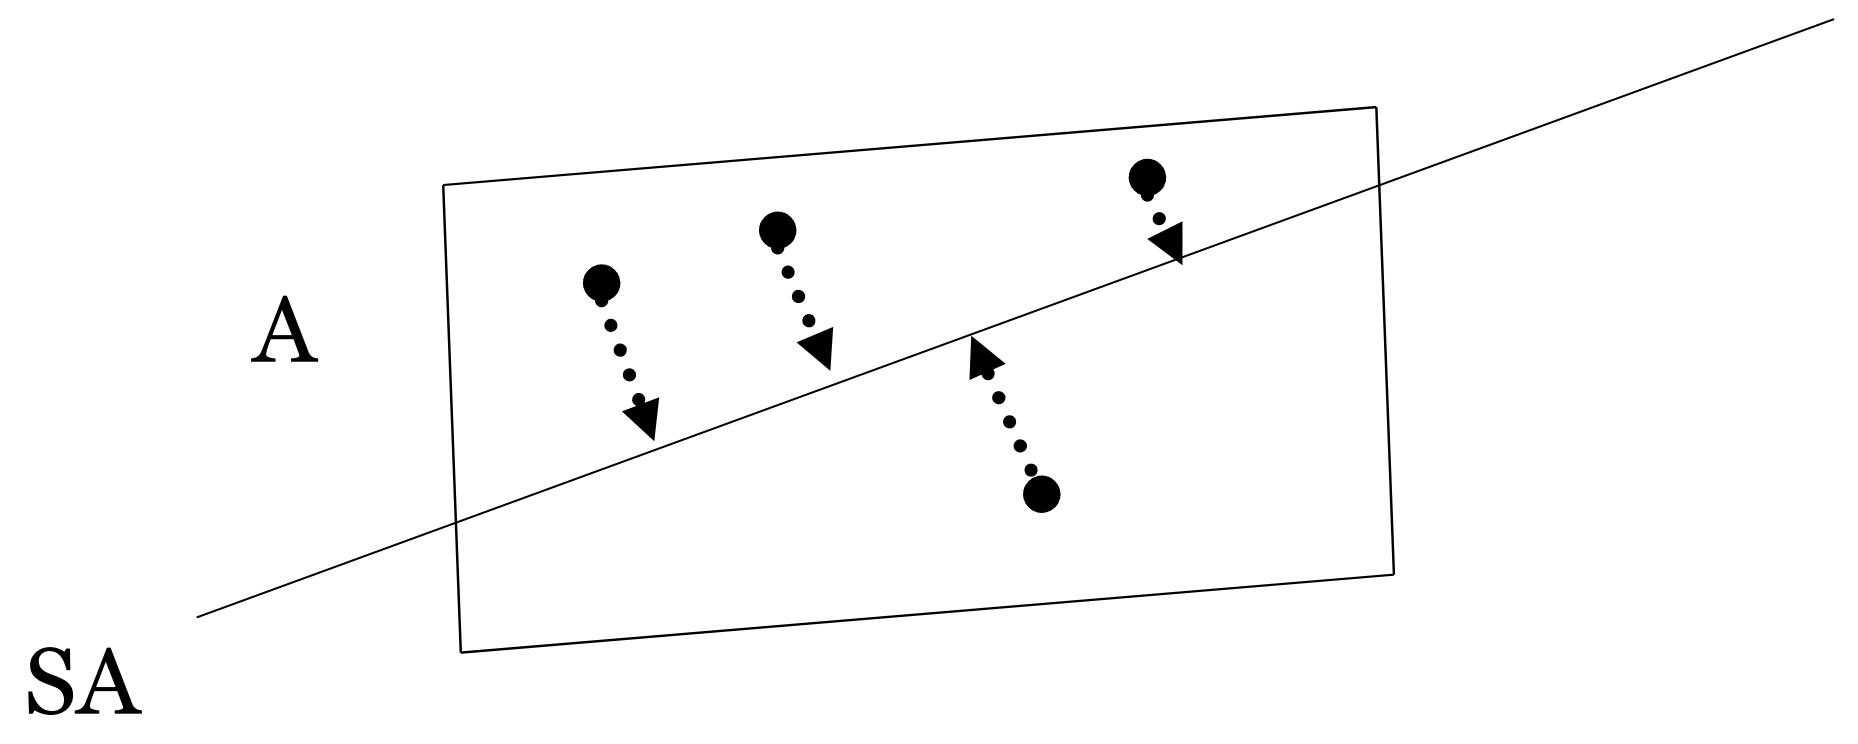
\includegraphics[width=0.6\textwidth]{images/2025-02-15-00-36-11.png}
      \end{center} 
\end{enum}

\section{First attempt: finding best approximation in rowspan $SA$}
We solve want the minimum of $\norm*{XSA - A}_{F} $ over rank $k$ $X$. Using the normal equations and Pythagorean theorem (think of this as over rows, where we can represent the distance from $X_i SA$ as the distance from $X_i SA$ to the optimum projection of $A_i $ onto $SA$, and the distance from the optimum to $A_i $):
\[
    \norm*{XSA - A}_{F} ^2  = \norm*{XSA - A(SA)^- SA}_{F} ^2 + \norm*{A(SA)^- SA - A}_{F}^2 . 
\]
So the minimizer of $X$ is 
\[
    \argmin_{X} \norm*{XSA - A(SA)^- SA}_{F}^2  . 
\]
Write $SA = U \Sigma V^{\top} $ in sparse form (so that $U\Sigma $ is square) then 
\begin{align*}
    \argmin_{X} \norm*{XSA - A(SA)^- SA}_{F}^2 &= \argmin_{X} \norm*{XU\Sigma  - A(SA)^- U \Sigma }_{F} \\
    &= \argmin_{Y} \norm*{Y - A(SA)^- U\Sigma }_{F} ,
\end{align*}
where the first equality comes from the fact that $V^{\top} $ has orthonormal rows, and the second equality comes from the fact that $U \Sigma $ is invertible. 

We can solve for the minimum now by taking SVD of $A(SA)^- U\Sigma $, but the problem is left multiplying by $A$, which takes $O(nnz(A) \poly(k/\eps ))$ (each row $A_i $ sums $nnz(A_i )$ rows of size $k/\eps $). We will address this by approximating the projection of $A$ onto $SA$ using affine embeddings. 

\section{Faster by approximating projection}
Let's revisit 
\[
    \min _X \norm*{XSA - A}_{F} ^2. 
\]
Let $R$ be a transposed CountSketch matrix with $k/\eps $ columns so that we can compute $AR$, $SAR$ in $O(nnz(A))$ time. We have the sketched problem guarantee: 
\[
    \norm*{XSAR - AR}_{F} \leq (1+\eps ) \norm*{XSA - A}_{F} . 
\]
Mirroring the earlier approach with Pythagorean theorem and a change of variables: 
\begin{align*}
    &\min _X \norm*{XSAR - AR}_{F} \\
    &=  \min _X \norm*{XSAR - AR(SAR)^- SAR}_{F} ^2  + \min _X \norm*{AR(SAR)^- SAR - AR}_{F}^2 \\
    &= \min _X \norm*{XSAR - AR(SAR)^- SAR}_{F} ^2\\
    &= \min _Y \norm*{Y - AR(SAR)^- SAR}_{F} ^2 . 
\end{align*}
Now, since $AR$ is $n \times k/\eps $ and $SAR$ is $k/\eps \times k/\eps $, we can compute $AR(SAR)^- SAR$ in $O(n (k/\eps )^2 )$, this time in bounds. The failure probability is constant by a union bound over constant failure probabilities of $S$ and $R$. In summary, the algorithm
\begin{enum}
    \item Compute $SA$ . 
    \item Compute $\min _Y \norm*{Y - AR(SAR)^- SAR}_{F} ^2$ with truncated SVD. 
    \item Output $Y(SAR)^- SA$ (in factored form to stay in complexity bounds). 
\end{enum}
achieves with constant failure probability a rank $k$ approximation of $A$ in time $O(nnz(A) + (n+d)\poly(d/\eps ))$. 


\end{document}